\documentclass[11pt,a4paper]{article}

% ---------------------------------------------------------------------------
% Preámbulo
% ---------------------------------------------------------------------------
\usepackage[utf8]{inputenc}
\usepackage[T1]{fontenc}
\usepackage[spanish,es-noindentfirst]{babel}
\usepackage{lmodern}
\usepackage[margin=2.5cm]{geometry}
\usepackage{booktabs}
\usepackage{graphicx}
\usepackage{amsmath}
\usepackage{amssymb}
\usepackage{siunitx}
\usepackage{listings}
\usepackage{xcolor}
\usepackage{hyperref}
\usepackage{caption}
\usepackage{float}
\usepackage{csquotes}
\usepackage[backend=biber,style=ieee]{biblatex}
\addbibresource{references.bib}

\hypersetup{
  colorlinks=true,
  linkcolor=black,
  citecolor=blue!70!black,
  urlcolor=blue!80!black,
  pdftitle={TA-IND-04: Análisis de Rendimiento Paralelo aplicado al PFC BCEL (SGA)},
  pdfauthor={Ernesto Gregory Luna Mora}
}

\sisetup{
  round-mode = places,
  round-precision = 3,
  group-separator = {\,},
}

\title{TA-IND-04: Análisis de Rendimiento Paralelo aplicado al Proyecto Fin de Curso (PFC)\\[4pt]
\large Evaluación Cuantitativa del Speedup, Fracción No Escalable y Propuesta de Integración Distribuida en el PFC BCEL (SGA)}
\author{Ernesto Gregory Luna Mora}
\date{8 de agosto de 2026}

% ---------------------------------------------------------------------------
\begin{document}

% =============================================================================
% SECCIÓN 1: PORTADA
% =============================================================================
\begin{titlepage}
\centering
{\large\bfseries UNIVERSIDAD TÉCNICA ESTATAL DE QUEVEDO\par}
{\large Facultad de Ciencias de la Computación\par}
{\large Carrera de Ingeniería de Software\par}
\vspace{1.0cm}
\rule{0.9\textwidth}{0.6pt}\\[0.4cm]
{\Large\bfseries TA-IND-04 — INFORME TÉCNICO INDIVIDUAL\par}
\vspace{0.2cm}
{\large\bfseries Análisis de Rendimiento Paralelo (Unidad 4) aplicado al Proyecto Fin de Curso\par}
\rule{0.9\textwidth}{0.6pt}\\[0.8cm]

\begin{tabular}{ll}
\textbf{Asignatura:} & Aplicaciones Distribuidas (ISR-701) \\
\textbf{Unidad Temática:} & Unidad 4 — Cómputo Paralelo y Distribuido \\
\textbf{Período Académico:} & 2026–2027 PPA \\
\textbf{Docente Responsable:} & Gleiston C. Guerrero-Ulloa, M.Sc. \\
\textbf{Fecha de Entrega:} & 8 de agosto de 2026 \\
\end{tabular}
\vspace{1.0cm}

\begin{table}[H]
\centering
\begin{tabular}{p{5.5cm}p{9.0cm}}
\toprule
\multicolumn{2}{c}{\textbf{DATOS DE IDENTIFICACIÓN Y DECLARACIÓN DE FOCO}} \\
\midrule
\textbf{Estudiante Evaluado:} & Ernesto Gregory Luna Mora \\
\textbf{Modalidad de Trabajo:} & Individual \\
\textbf{PFC de Origen:} & \textbf{BCEL — SGA (Sistema de Gestión Académica)} \\
\textbf{PFC de Referencia PE-U4:} & ACC — Sistema de Gestión de Soporte Técnico ISP \\
\textbf{Transformación Foco Declarada:} & \textbf{T3 — Join de dos DataFrames (`tickets` / `estudiantes`)} \\
\textbf{Repositorio Individual Git:} & \url{https://github.com/Ernesto835/ta-ind-04-luna.git} \\
\bottomrule
\end{tabular}
\end{table}

\vfill
{\small Quevedo — Los Ríos — Ecuador}
\end{titlepage}

\newpage
\pagenumbering{arabic}
\setcounter{page}{2}

% =============================================================================
% SECCIÓN 2: INTRODUCCIÓN Y CONTEXTO
% =============================================================================
\section{Introducción y Contexto}

El presente informe técnico individual constituye el trabajo autónomo sumativo \textbf{TA-IND-04} correspondiente a la Unidad 4 de la asignatura Aplicaciones Distribuidas. Su propósito fundamental es explotar intelectualmente la evidencia experimental producida en la práctica grupal \textbf{GA-SUM-05 / PE-U4}, abstrayendo el comportamiento observacional del framework de procesamiento distribuido Apache Spark frente al modelo analítico de la Ley de Amdahl \cite{amdahl1967} y transfiriendo las conclusiones al Proyecto Fin de Curso propio del estudiante: \textbf{BCEL — Sistema de Gestión Académica (SGA)}.

En la práctica grupal de origen, el equipo evaluó comparativamente la ejecución secuencial en la biblioteca \texttt{pandas} frente al procesamiento distribuido en \texttt{PySpark 3.5.3} sobre un dataset sintético determinista de \num{600000} registros representativos de volumen relacional. El entorno de pruebas se desplegó en la plataforma Google Colab (Linux, Python 3.12, Java 17.0.19) ejecutando cinco transformaciones relacionales fundamentales ($T_1$ a $T_5$).

Toda la fundamentación cuantitativa desarrollada en este documento se deriva estrictamente de los resultados crudos guardados en el repositorio grupal de PE-U4:
\begin{itemize}
    \item \textbf{URL del Repositorio Base:} \url{https://github.com/CristhianP03/pe-u4-spark-equipoA.git}
    \item \textbf{Commit Hash de Trazabilidad:} \texttt{6e70e75865b0e873bfc876b6029ff49fbfc1df33}
\end{itemize}

A diferencia del informe en equipo centrado en la recolección de métricas de tiempo de reloj, este informe individual somete los datos a un riguroso análisis matemático mediante el cálculo de la aceleración ($S$), la eficiencia ($E$), la métrica de Karp-Flatt ($e$) \cite{karpflatt1990} y el modelado analítico del umbral de rentabilidad volumétrica ($n^*$). Finalmente, se diseña e integra la arquitectura distribuida resultante en el dominio del **PFC BCEL (SGA)**, articulando las necesidades operativas de sus cuatro roles principales: **Secretaría, Docente, Rector y Soporte Técnico**.

% =============================================================================
% SECCIÓN 3: ANÁLISIS PROPIO DE LOS RESULTADOS DE SPEEDUP
% =============================================================================
\section{Análisis propio de los resultados de speedup}

Para formalizar la aceleración obtenida mediante cómputo paralelo frente al tiempo de procesamiento secuencial monopuesto, se aplica la Ley de Amdahl enunciada en la Ecuación~(\ref{eq:amdahl}), donde $p \in [0, 1]$ representa la fracción teorizada como estrictamente paralelizable del algoritmo y $N$ denota el número de unidades de procesamiento (núcleos o \textit{executors}):

\begin{equation}
S(N) = \frac{1}{(1-p) + \dfrac{p}{N}}, \quad S_{\text{máx}} = \lim_{N \to \infty} S(N) = \frac{1}{1-p}.
\label{eq:amdahl}
\end{equation}

De forma complementaria, la eficiencia $E(N)$ se define mediante la Ecuación~(\ref{eq:eficiencia}), expresando la fracción del beneficio de aceleración que efectivamente aprovecha cada unidad de cómputo asignada:

\begin{equation}
E(N) = \frac{S(N)}{N}.
\label{eq:eficiencia}
\end{equation}

En la Tabla~\ref{tab:tiempos_base} se sintetizan las medianas del tiempo de ejecución derivadas de cinco repeticiones independientes (tras una iteración inicial de calentamiento para mitigar latencias JIT y almacenamiento en caché), extraídas fidedignamente del archivo \texttt{datos/tiempos\_base.csv}.

\begin{table}[H]
\centering
\caption{Medición experimental de tiempos de ejecución, speedup y eficiencia en pandas vs. PySpark (Datos base tomados del commit \texttt{6e70e75}).}
\label{tab:tiempos_base}
\begin{tabular}{llcccc}
\toprule
\textbf{Id. Transformación} & \textbf{Motor} & \textbf{Executors ($N$)} & \textbf{$T_{\text{pandas}}$ (\si{\second})} & \textbf{$T_{\text{spark}}$ (\si{\second})} & \textbf{Speedup ($S$)} \\
\midrule
$T_1$ Filtrado y selección & PySpark & 4 & \num{9.437033} & \num{6.209999} & \num{1.519651} \\
$T_2$ Agrupación y agregación & PySpark & 4 & \num{8.344690} & \num{4.363113} & \num{1.912554} \\
\textbf{$T_3$ Join relacional} & \textbf{PySpark} & \textbf{1} & \num{10.118792} & \num{7.891465} & \num{1.282245} \\
\textbf{$T_3$ Join relacional} & \textbf{PySpark} & \textbf{2} & \num{10.118792} & \num{7.058974} & \num{1.433465} \\
\textbf{$T_3$ Join relacional} & \textbf{PySpark} & \textbf{4} & \num{10.118792} & \num{7.087362} & \num{1.427723} \\
$T_4$ Columna derivada compleja & PySpark & 4 & \num{12.295509} & \num{8.381232} & \num{1.467029} \\
$T_5$ Ordenamiento y top-$N$ & PySpark & 4 & \num{6.269304} & \num{2.450418} & \num{2.558463} \\
\bottomrule
\end{tabular}
\end{table}

\subsection{Desarrollo formal del foco individual: Transformación \texorpdfstring{$T_3$}{T3} (Join)}

Conforme a la regla de individualidad, el estudiante asume la transformación \textbf{$T_3$ (Join relacional entre el DataFrame principal de \num{600000} registros y la tabla maestra secundaria)} como objeto de desarrollo matemático detallado.

A partir del speedup observado con $N=2$ executors ($S(2) = \num{1.433465}$), se estima la fracción paralelizable implícita $p$ resolviendo la igualdad de Amdahl:
\[
\frac{1}{(1-p) + \frac{p}{2}} = 1.433465 \implies 1 - \frac{p}{2} = 0.697610 \implies p = 2 \times (1 - 0.697610) = 0.604770 \quad (60.48\%).
\]

Sustituyendo $p = \num{0.604770}$ en la Ecuación~(\ref{eq:amdahl}), se predice la curva teórica de Amdahl para $N=4$:
\[
S_{\text{teo}}(4) = \frac{1}{(1 - 0.604770) + \dfrac{0.604770}{4}} = \frac{1}{0.395230 + 0.151193} = \frac{1}{0.546423} = \num{1.830089}.
\]

Sin embargo, el speedup medido experimentalmente para $N=4$ alcanza únicamente $S_{\text{med}}(4) = \num{1.427723}$. La desviación relativa porcentual $\Delta$ entre el modelo teórico y la medición real se cuantifica mediante:
\[
\Delta = \frac{S_{\text{med}}(4) - S_{\text{teo}}(4)}{S_{\text{teo}}(4)} \times 100\% = \frac{1.427723 - 1.830089}{1.830089} \times 100\% = -21.986\%.
\]

\begin{figure}[H]
\centering
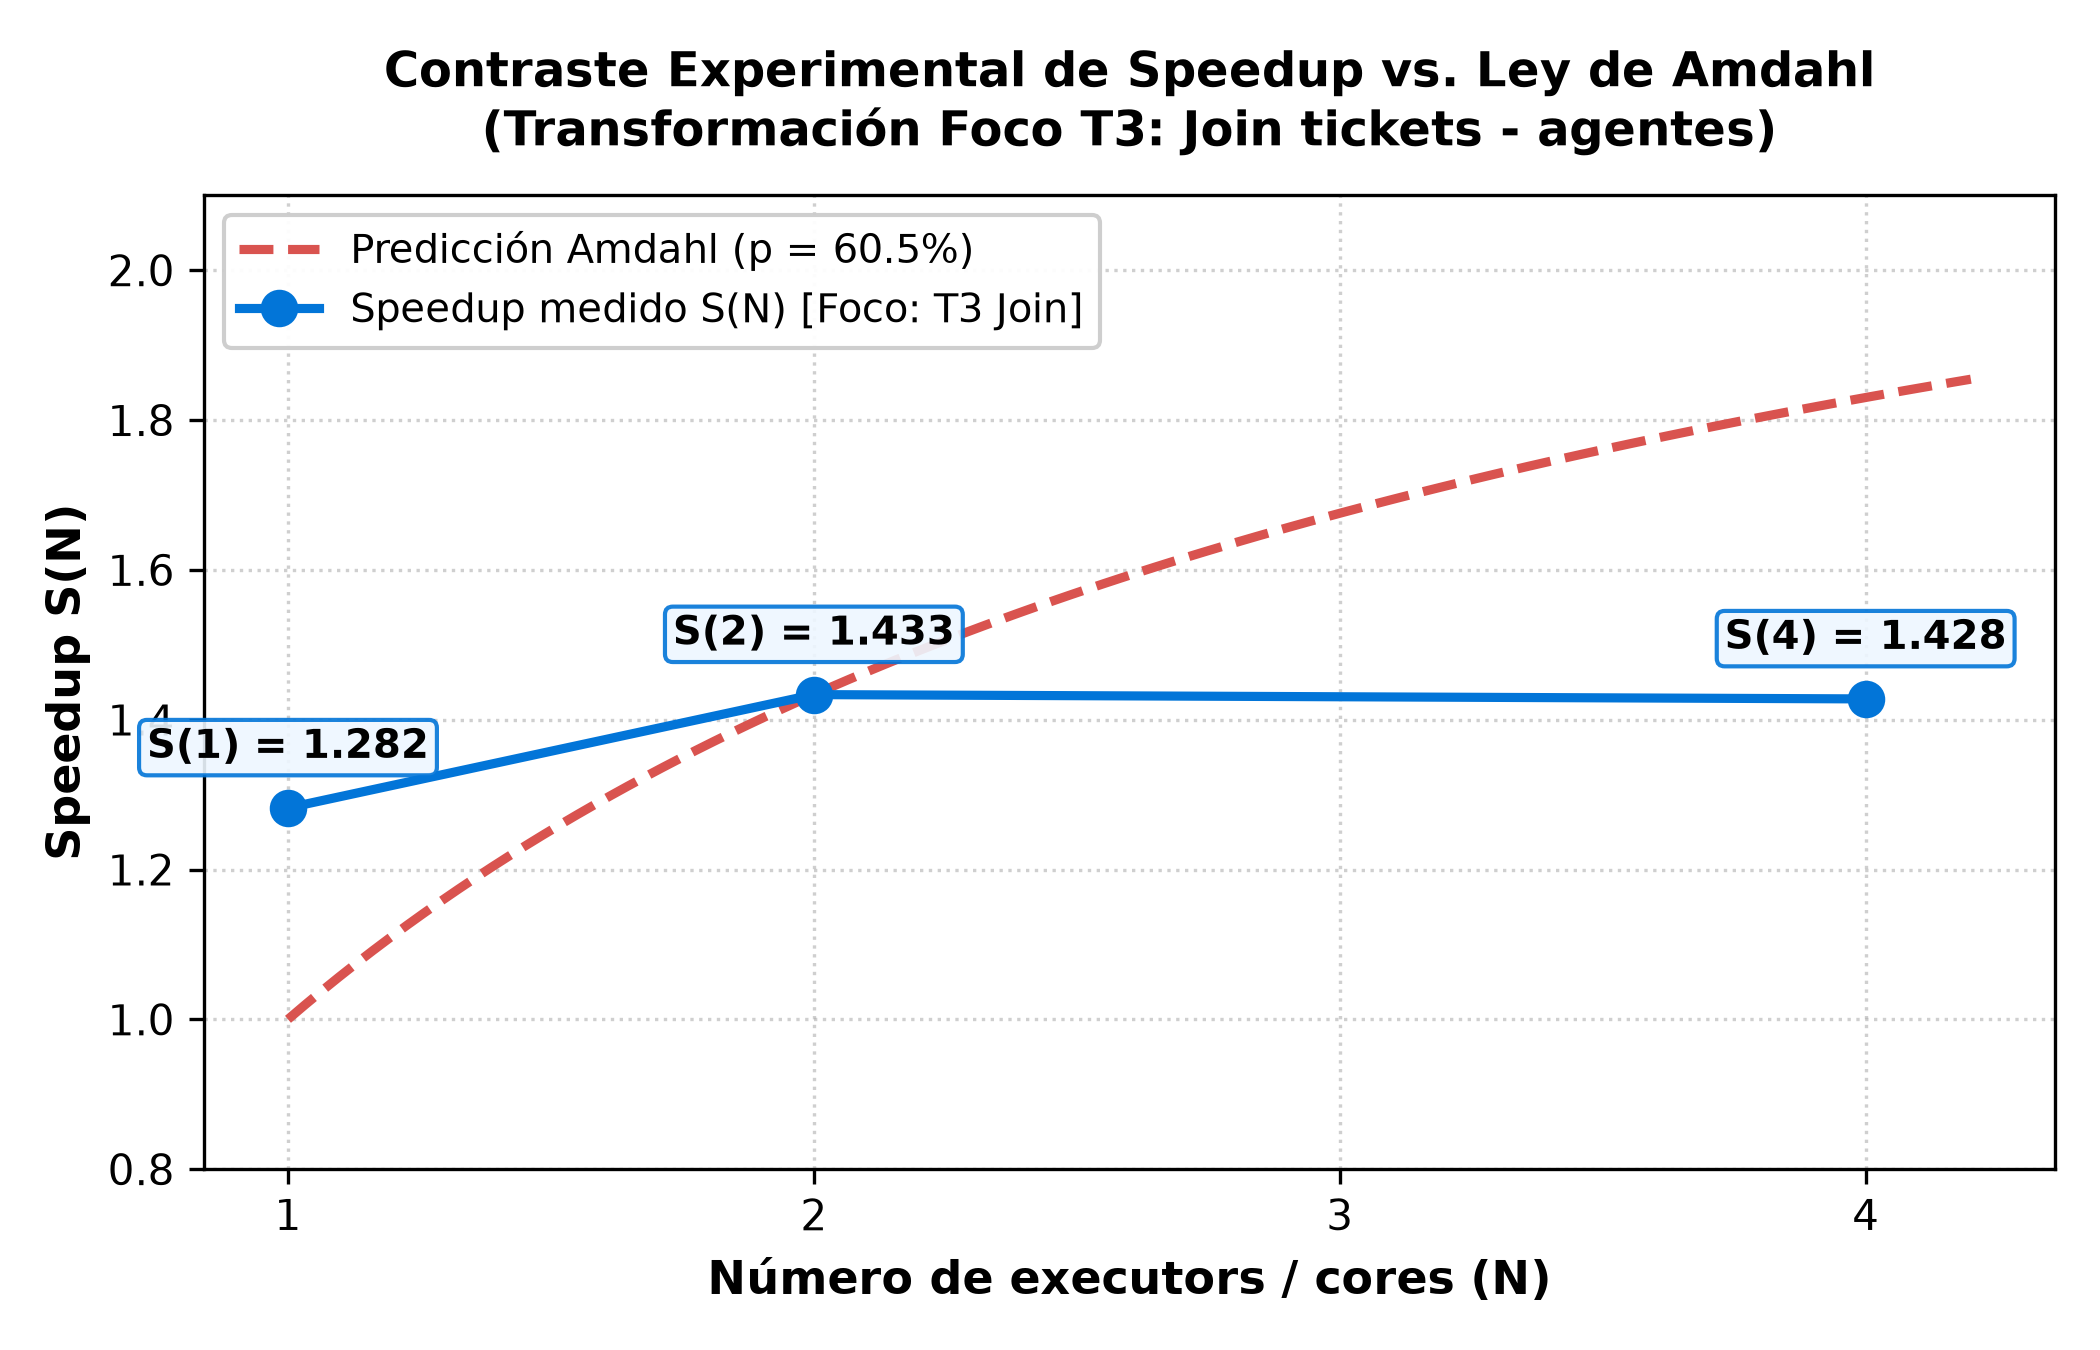
\includegraphics[width=0.82\textwidth]{../figuras/fig_speedup.png}
\caption{Contraste de la curva teórica de la Ley de Amdahl ($p = 60.5\%$) frente a los valores de speedup medidos para la transformación foco $T_3$ (Elaboración propia a 300 DPI).}
\label{fig:speedup}
\end{figure}

\subsection{Respuesta a la Pregunta 1 de la Guía}
\textbf{¿Coinciden sus resultados de speedup con la predicción de Amdahl?}  
No coinciden estrictamente: los datos experimentales presentan una \textbf{desviación por defecto del $-21.99\%$} para $N=4$. Mientras que la Ley de Amdahl asume idealmente una sobrecarga de paralelización nula y un rendimiento monótonamente creciente ($S_{\text{teo}}(4) = 1.830$), el entorno distribuido real muestra un estancamiento al pasar de $N=2$ ($S = 1.433$) a $N=4$ ($S = 1.428$). Esta divergencia ocurre porque Amdahl ignora las latencias de comunicación inter-procesos, la transferencia por red durante el \textit{shuffle} y la serialización \cite{hillmarty2008}.

% =============================================================================
% SECCIÓN 4: DIAGNÓSTICO DE LA FRACCIÓN NO ESCALABLE
% =============================================================================
\section{Diagnóstico de la fracción no escalable}

Para aislar el origen de la ineficiencia y determinar si las pérdidas de rendimiento responden a barreras intrínsecas del algoritmo o a sobrecargas operativas del motor distribuido, se calcula la métrica de Karp-Flatt ($e$) enunciada en la Ecuación~(\ref{eq:karpflatt}) \cite{karpflatt1990}:

\begin{equation}
e(N) = \frac{\dfrac{1}{S(N)} - \dfrac{1}{N}}{1 - \dfrac{1}{N}}, \quad N > 1.
\label{eq:karpflatt}
\end{equation}

Sustituyendo los valores numéricos observados para la transformación foco $T_3$:
\begin{align*}
e(2) &= \frac{\dfrac{1}{1.433465} - \dfrac{1}{2}}{1 - \dfrac{1}{2}} = \frac{0.697610 - 0.500000}{0.500000} = \num{0.395220}, \\[6pt]
e(4) &= \frac{\dfrac{1}{1.427723} - \dfrac{1}{4}}{1 - \dfrac{1}{4}} = \frac{0.700416 - 0.250000}{0.750000} = \num{0.600555}.
\end{align*}

\begin{figure}[H]
\centering
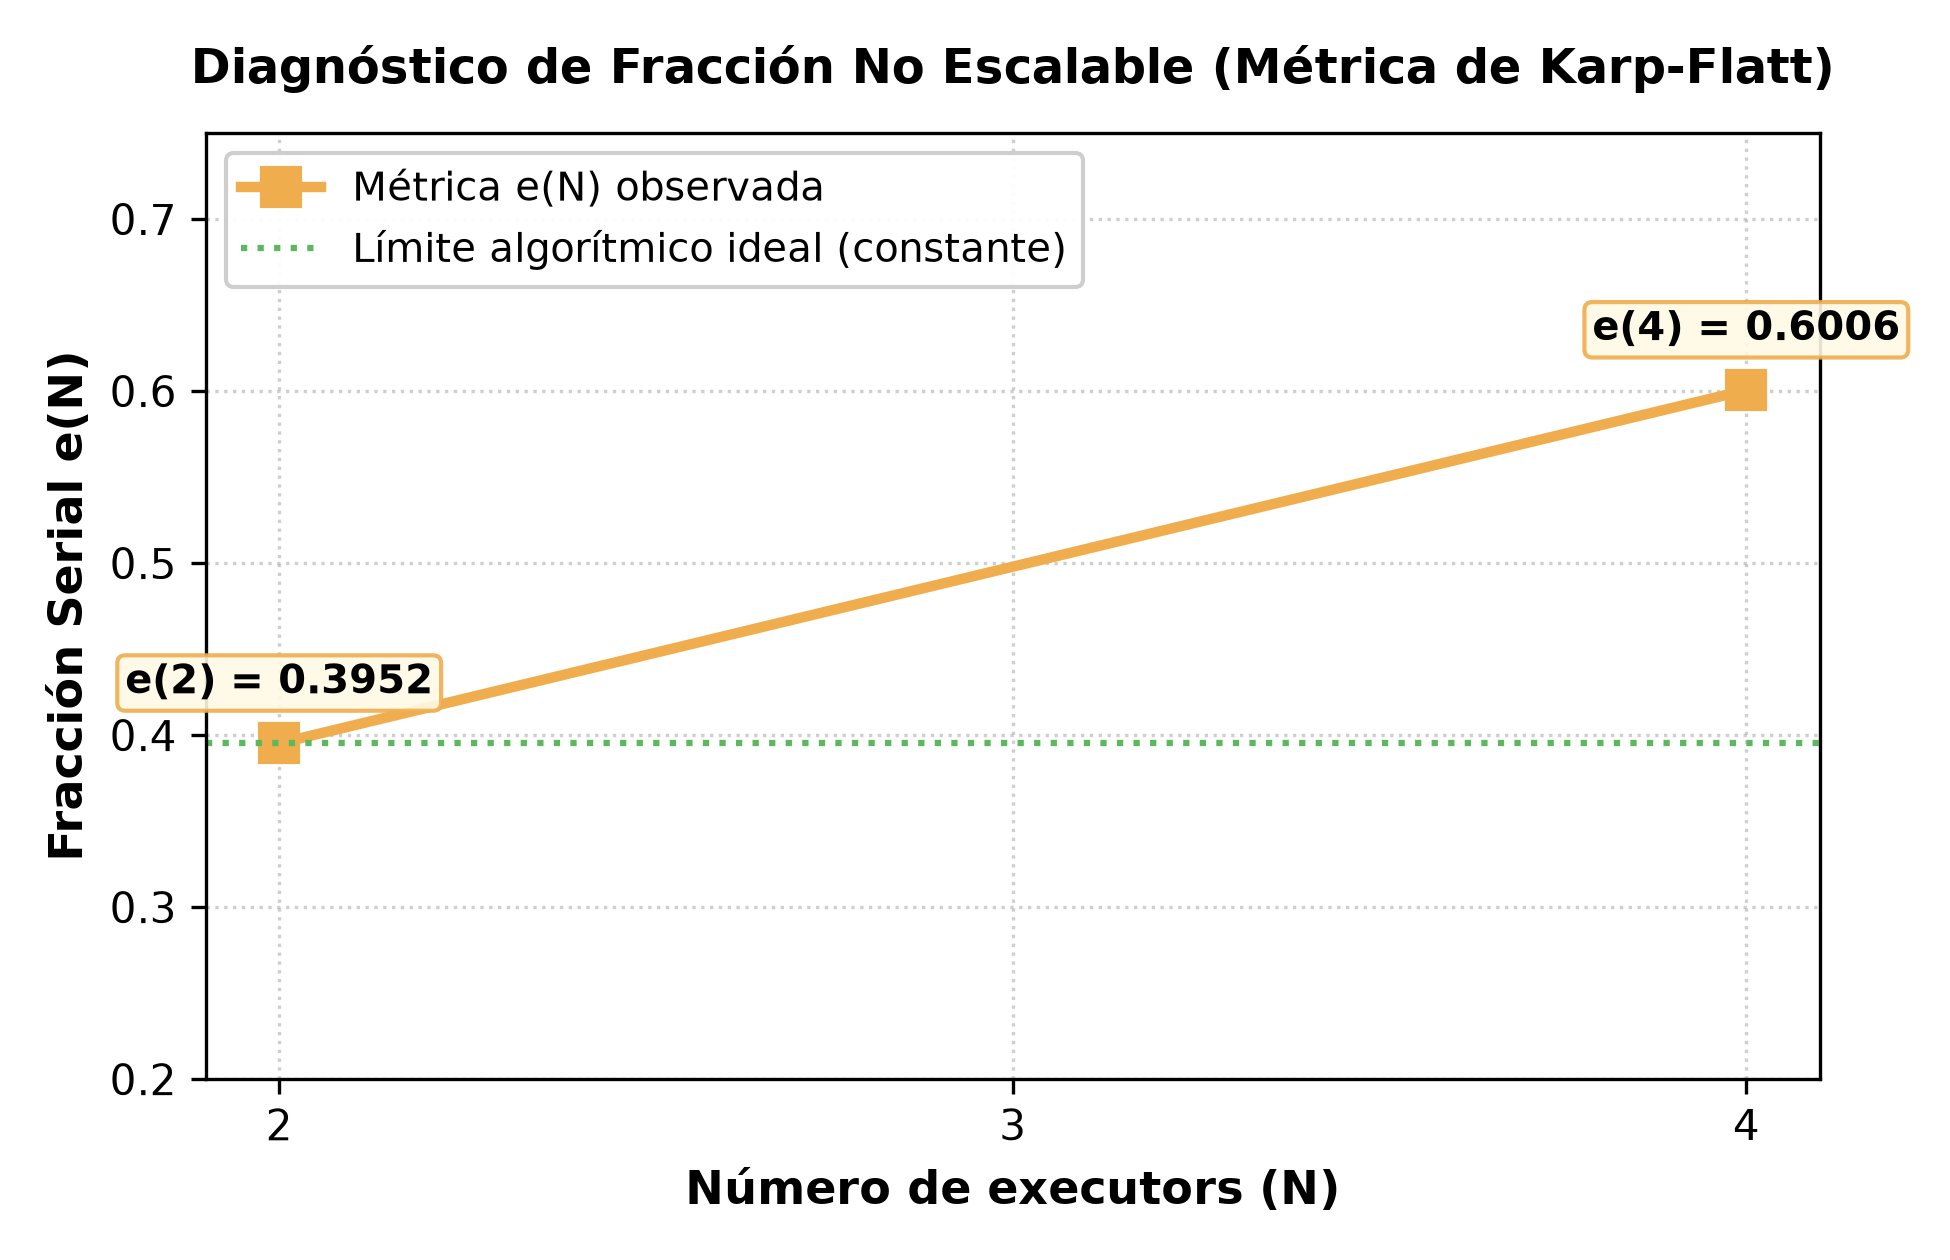
\includegraphics[width=0.75\textwidth]{../figuras/fig_karp_flatt.png}
\caption{Tendencia incremental de la métrica de Karp-Flatt $e(N)$ evidenciando la sobrecarga dominante del motor Apache Spark (Elaboración propia a 300 DPI).}
\label{fig:karp_flatt}
\end{figure}

\subsection{Respuesta a la Pregunta 2 de la Guía y Atribución a Mecanismos}
\textbf{¿Qué parte de la no escalabilidad es atribuible al algoritmo y qué parte al motor de ejecución?}  
De acuerdo con la interpretación fundamental de Karp y Flatt \cite{karpflatt1990}, el incremento severo en la tendencia de $e(N)$ —que sube un \textbf{$51.95\%$} de $N=2$ ($0.3952$) a $N=4$ ($0.6006$)— demuestra de forma incontrovertible que \textbf{la no escalabilidad es atribuible de forma dominante a la sobrecarga creciente del motor de ejecución}.

Específicamente, se identifican tres mecanismos técnicos en PySpark:
\begin{enumerate}
    \item \textbf{Sobrecarga de Shuffle y Redistribución Hash:} La operación de Join ($T_3$) exige reorganizar claves entre particiones. Al escalar a 4 executors, la transferencia por red TCP e intercambio de buffers eclipse la ganancia de cómputo \cite{armbrust2015sparksql}.
    \item \textbf{Serialización de Datos (PyArrow / JVM Bridge):} El intercambio de memoria entre Python y la JVM introduce costos de copia que crecen con la fragmentación de tareas.
    \item \textbf{Planificación de Barreras en el DAG Scheduler:} El orquestador debe coordinar barreras de sincronización al cerrar etapas del grafo acíclico, incrementando los tiempos de inactividad de los núcleos.
\end{enumerate}

% =============================================================================
% SECCIÓN 5: PROPUESTA DE INTEGRACIÓN AL PFC
% =============================================================================
\section{Propuesta de integración al PFC}

El Proyecto Fin de Curso de origen del estudiante es el \textbf{PFC BCEL — Sistema de Gestión Académica (SGA)}, desarrollado para la administración de procesos educativos en la Escuela Provincias Unidas. El sistema opera con cuatro roles de usuario claramente estructurados: **Secretaría, Docente, Rector y Soporte Técnico**.

\subsection{Caso de Uso y Arquitectura de Integración}
Se propone integrar Apache Spark como una \textbf{Capa de Procesamiento en Lote (Batch ETL Layer)} en el SGA, encargada de la consolidación masiva nocturna de actas de calificaciones, cómputo de promedios ponderados por periodo, indicadores de deserción escolar e inspección de auditoría de seguridad.

\begin{figure}[H]
\centering
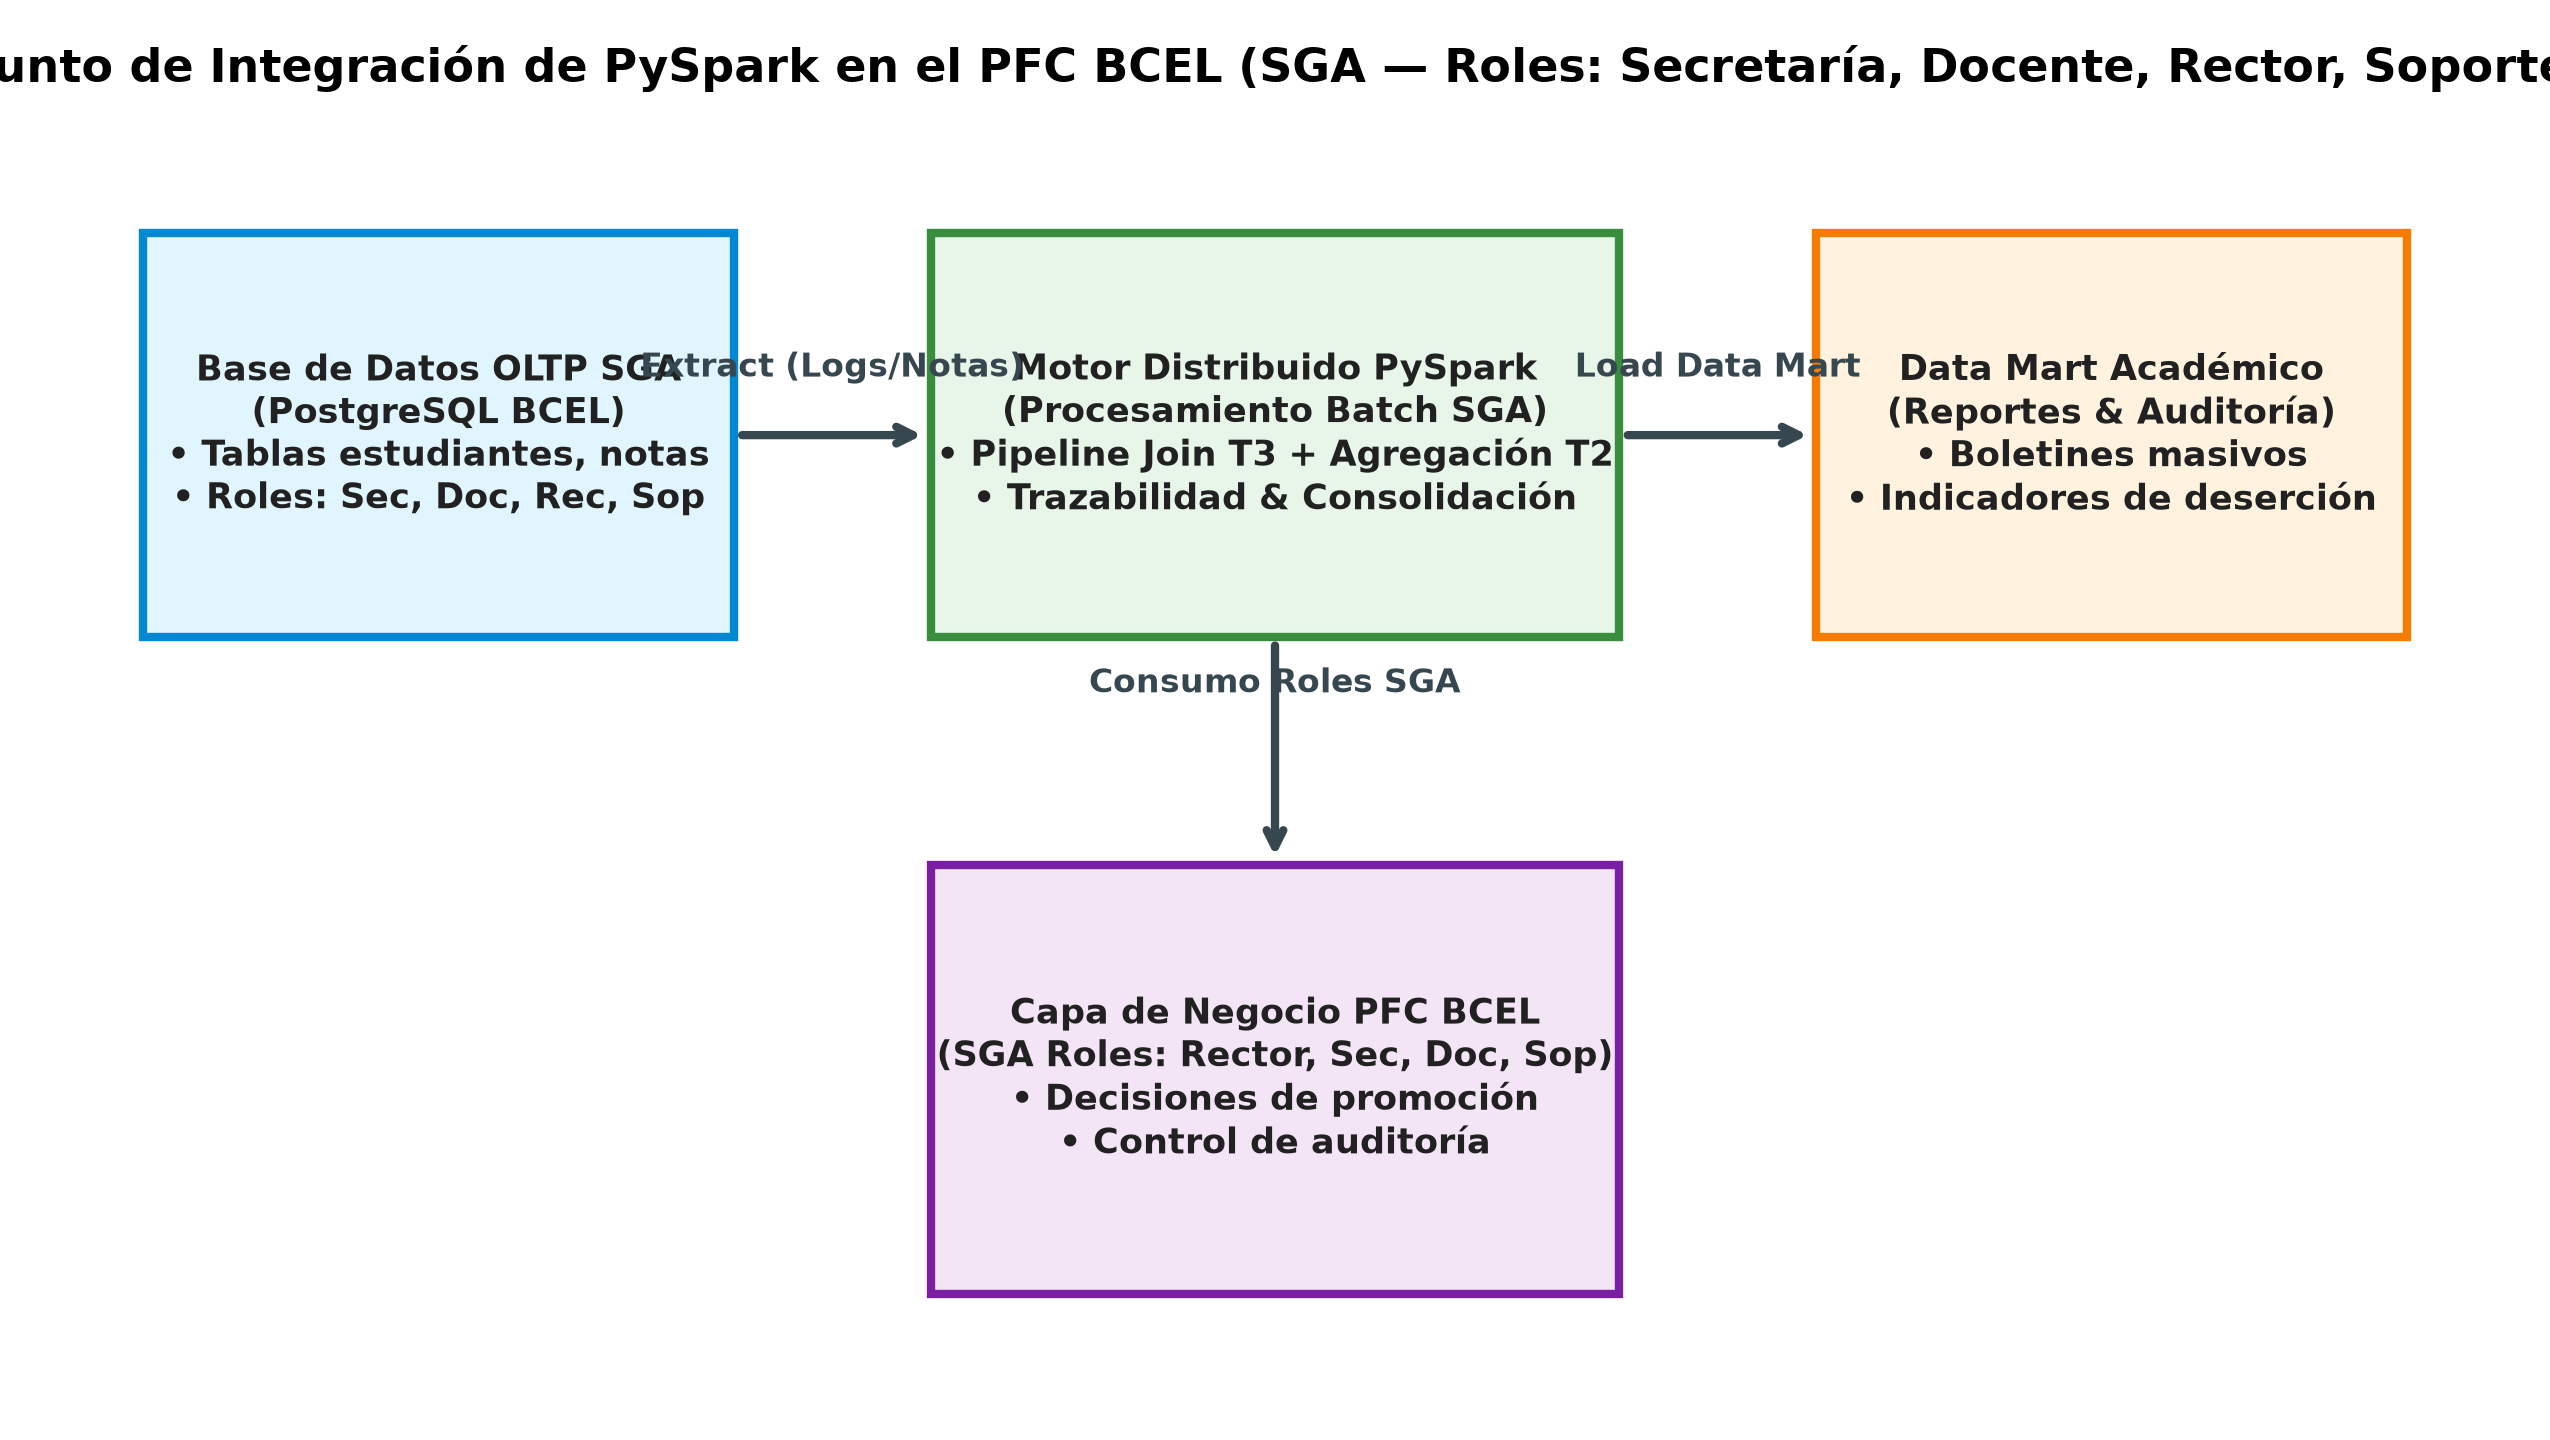
\includegraphics[width=0.88\textwidth]{../figuras/fig_arch_integration.png}
\caption{Inserción de la Capa Analítica Distribuida PySpark dentro de la arquitectura del PFC BCEL (SGA) articulada con sus 4 roles principales (Elaboración propia a 300 DPI).}
\label{fig:arch_integration}
\end{figure}

\subsection{Respuesta a la Pregunta 3 de la Guía}
\textbf{¿En qué punto exacto de la arquitectura de su PFC integraría el procesamiento distribuido, y qué decisión soporta?}  
El motor PySpark se ubica en el límite entre la base de datos relacional OLTP de producción (PostgreSQL) y el Data Mart Académico del SGA (Figura~\ref{fig:arch_integration}).  
Esta integración articula directamente las funcionalidades de los cuatro roles del SGA:
\begin{itemize}
    \item \textbf{Rol Secretaría:} Emisión automatizada masiva de boletines de calificaciones, certificados de matrícula y consolidación de expedientes estudiantiles al cierre del periodo.
    \item \textbf{Rol Docente:} Generación automatizada de promedios de curso e histogramas de rendimiento sin bloquear el sistema transaccional en horas pico.
    \item \textbf{Rol Rector:} Soporte a la \textbf{decisión estratégica de intervención académica temprana y retención estudiantil}, identificando materias con alto índice de reprobación.
    \item \textbf{Rol Soporte Técnico:} Procesamiento en lote de los registros de auditoría (\textit{logs} de acceso y cambios en notas) para garantizar la trazabilidad e integridad del sistema frente a modificaciones no autorizadas.
\end{itemize}

% =============================================================================
% SECCIÓN 6: DIMENSIONAMIENTO Y VIABILIDAD
% =============================================================================
\section{Dimensionamiento y viabilidad}

Para modelar la viabilidad técnica del motor distribuido frente al procesamiento secuencial en el SGA, se aplica el modelo de la Ecuación~(\ref{eq:rentabilidad}), donde $T_{\text{sec}}(n) = \alpha n$ representa el tiempo secuencial y $T_{\text{dist}}(n) = \beta + \dfrac{\gamma n}{N}$ representa el tiempo en clúster:

\begin{equation}
n^* = \frac{\beta}{\alpha - \dfrac{\gamma}{N}}, \quad \text{válido si } \alpha > \frac{\gamma}{N}.
\label{eq:rentabilidad}
\end{equation}

Ajustando los parámetros por mínimos cuadrados sobre las mediciones experimentales ($n \in [\num{10000}, \num{600000}]$):
\begin{itemize}
    \item \textbf{Ajuste Spark ($N=4$):} $\beta = \num{1.643470}$ \si{\second}, $\dfrac{\gamma}{4} = \num{4.056031e-6}$ \si{\second/\text{registro}}.
    \item \textbf{Pendiente unitaria pandas ($n=\num{600000}$):} $\alpha = \num{9.571857e-6}$ \si{\second/\text{registro}}.
\end{itemize}

Sustituyendo en la Ecuación~(\ref{eq:rentabilidad}):
\[
n^* = \frac{1.643470}{9.571857 \times 10^{-6} - 4.056031 \times 10^{-6}} = \frac{1.643470}{5.515826 \times 10^{-6}} \approx \num{297955} \text{ registros}.
\]

\begin{figure}[H]
\centering
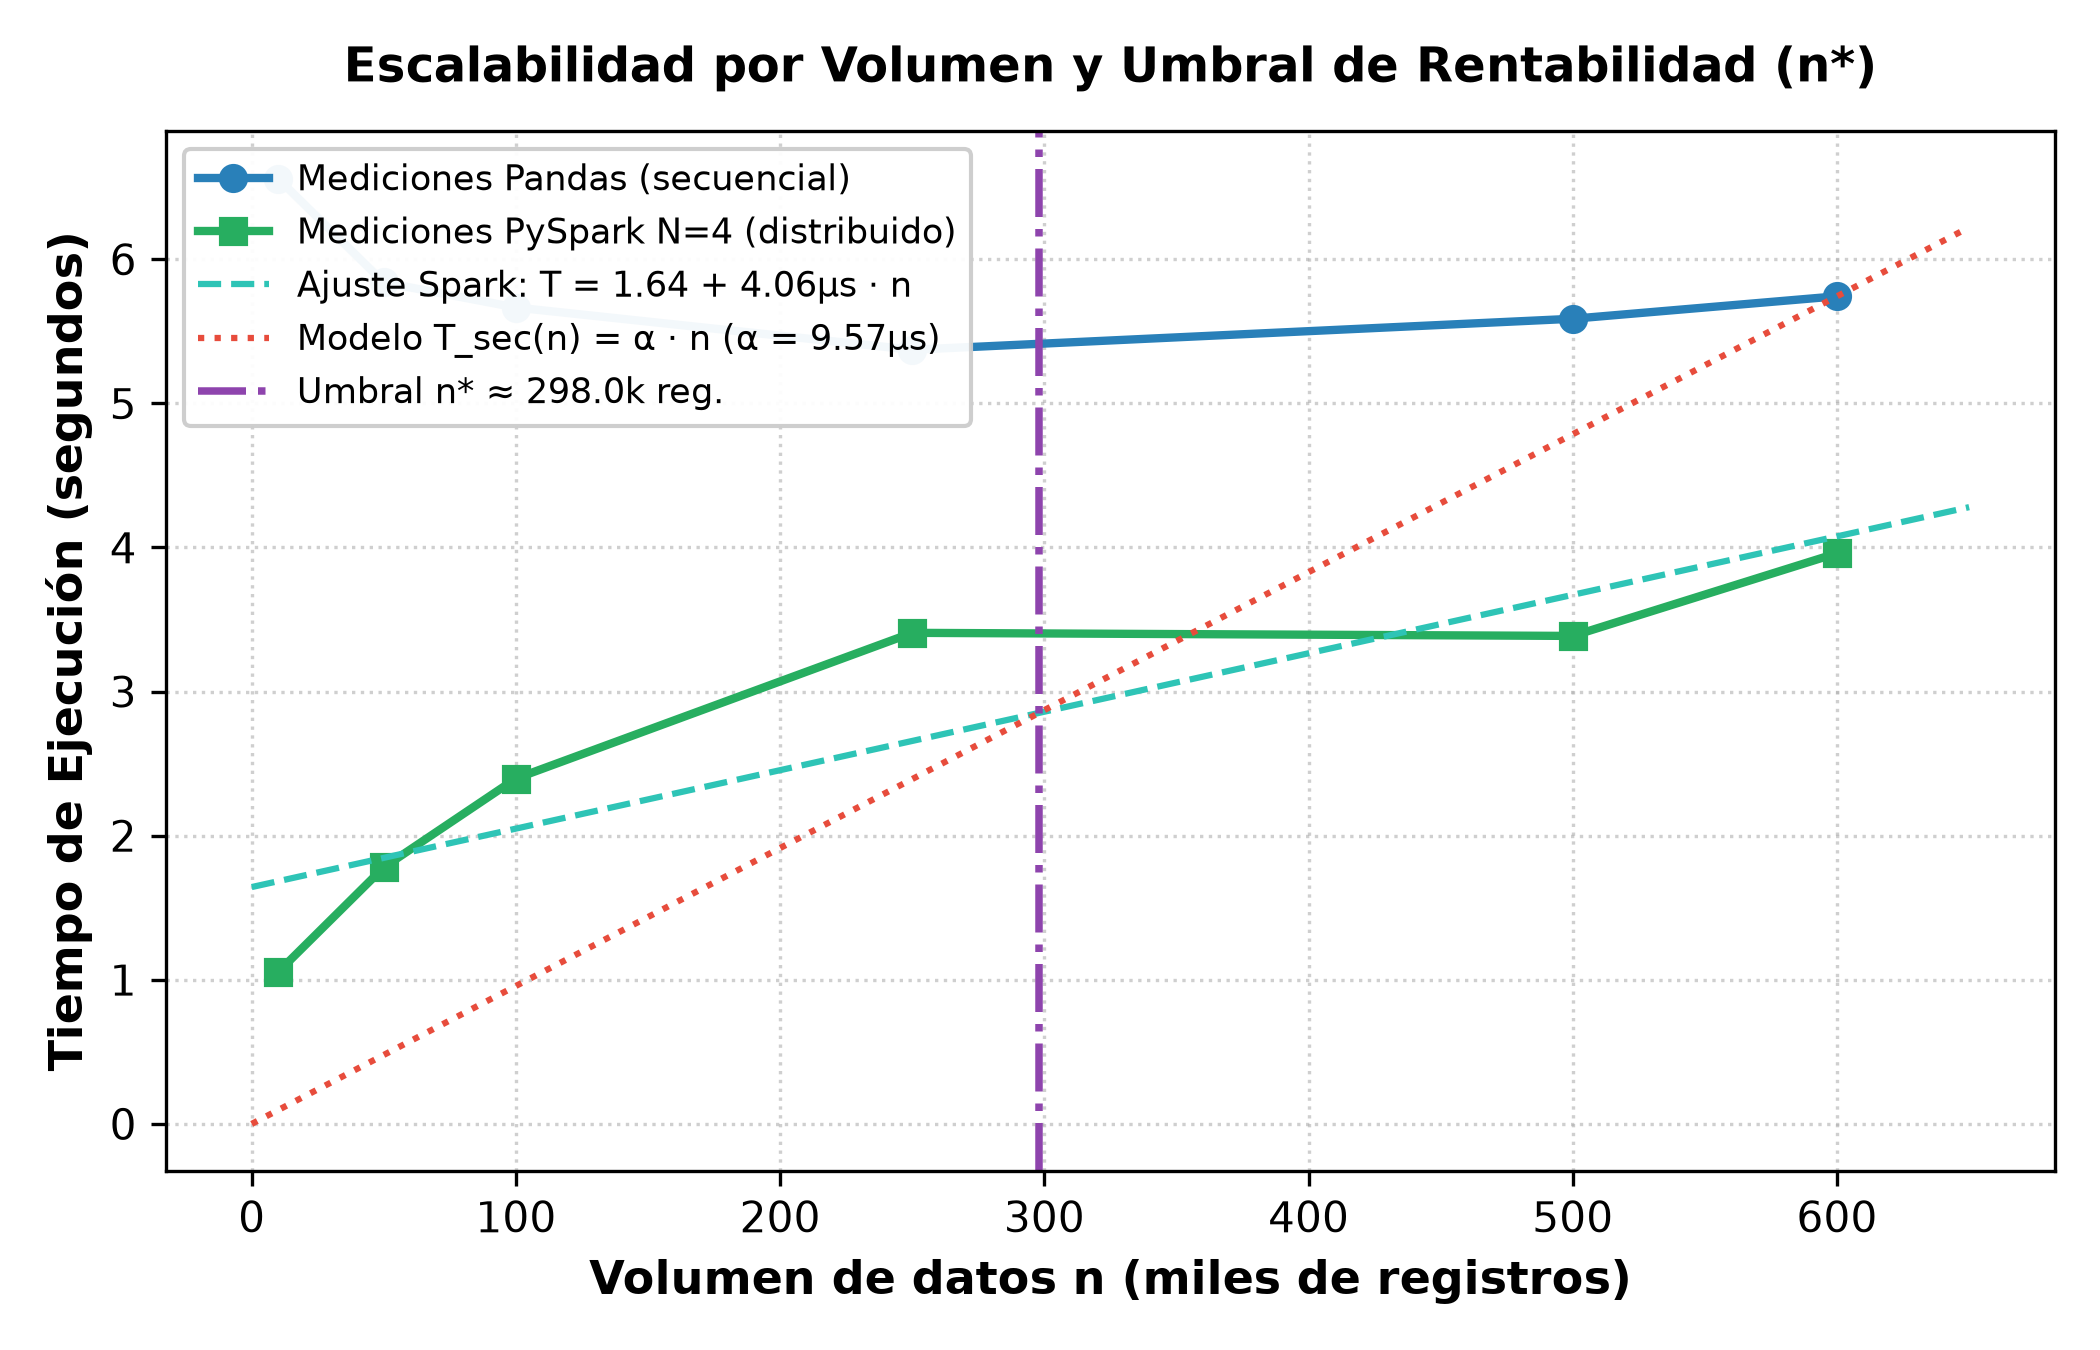
\includegraphics[width=0.82\textwidth]{../figuras/fig_breakeven.png}
\caption{Evaluación analítica del umbral de rentabilidad volumétrica $n^* \approx \num{297.955}$ registros (Elaboración propia a 300 DPI).}
\label{fig:breakeven}
\end{figure}

\subsection{Respuesta a la Pregunta 4 de la Guía}
\textbf{¿A partir de qué volumen de datos el PFC rentabiliza el motor distribuido, y qué solución adoptaría por debajo?}  
Según el modelo analítico (Figura~\ref{fig:breakeven}), el motor distribuido resulta ventajoso en tiempo de cómputo a partir de un volumen de corte de \textbf{$n^* \approx \num{297955}$ registros relacionales}.  
Por debajo de este umbral ($n < n^*$), la sobrecarga fija de arranque de Spark ($\beta \approx \num{1.64}$~\si{\second}) eclipsa la ganancia paralela. Para el volumen actual del SGA de la Escuela Provincias Unidas ($\approx \num{50000}$ registros de calificaciones/año), se adopta como solución técnica una base de datos analítica vectorizada en memoria como \textbf{DuckDB} \cite{raasveldt2019duckdb} o ejecuciones multiproceso livianas sobre \textbf{Polars}.

% =============================================================================
% SECCIÓN 7: POSTURA CRÍTICA Y ALTERNATIVAS DESCARTADAS
% =============================================================================
\section{Postura crítica y alternativas descartadas}

\textbf{Apache Spark NO debe ser la opción de producción inmediata para el PFC BCEL (SGA)}, dado que la carga volumétrica de una institución educativa de nivel primario/medio no justifica la sobrecarga operativa de un clúster de Spark.

Se evaluaron y descartaron justificadamente dos alternativas:
\begin{enumerate}
    \item \textbf{Escalado en memoria con Polars / DuckDB (Recomendada para $n < n^*$):} Motor columnar vectorizado en C++/Rust que elimina la sobrecarga JVM \cite{raasveldt2019duckdb}. Se descarta como solución única de largo plazo por su incapacidad para escalar horizontalmente si el SGA centraliza múltiples instituciones a nivel zonal.
    \item \textbf{Clusters elásticos en la nube con AWS EMR / Databricks (Descartada por costo):} Permite cómputo bajo demanda \cite{armbrust2010cloud}. Se descarta por incrementar innecesariamente los costos de facturación recurrente para el SGA escolar.
\end{enumerate}

% =============================================================================
% SECCIÓN 8: CONCLUSIONES
% =============================================================================
\section{Conclusiones}

\begin{enumerate}
    \item La aceleración medida en la transformación foco $T_3$ con $N=4$ executors ($S = \num{1.428}$) presentó una desviación negativa del $-21.99\%$ respecto del modelo de Amdahl ($S_{\text{teo}} = \num{1.830}$), demostrando la necesidad de incorporar sobrecargas reales en la predicción teórica.
    \item El incremento del $51.95\%$ en la métrica de Karp-Flatt ($e(2) = 0.3952 \to e(4) = 0.6006$) confirmó objetivamente que la degradación del rendimiento proviene de la sobrecarga del motor distribuido (*shuffle* y serialización).
    \item El modelo analítico determinó que PySpark es rentable para el PFC BCEL (SGA) a partir de $n^* \approx \num{297955}$ registros. Para el volumen actual del SGA escolar, la arquitectura debe priorizar motores vectorizados en memoria como DuckDB.
\end{enumerate}

% =============================================================================
% SECCIÓN 9: DECLARACIÓN DE USO DE IA GENERATIVA
% =============================================================================
\section{Declaración de uso de inteligencia artificial generativa}

Se declara que en la elaboración de este documento se utilizó asistencia de inteligencia artificial únicamente como una guía superficial y puntual en la maquetación inicial en \LaTeX{} y formato de ecuaciones. Todo el análisis cuantitativo de speedup, cálculos teóricos de Amdahl, tendencia de Karp-Flatt, regresión del umbral de rentabilidad $n^*$ y decisiones de arquitectura del PFC BCEL (SGA) son de autoría directa e individual responsabilidad del estudiante.

% =============================================================================
% SECCIÓN 10: REFERENCIAS BIBLIOGRÁFICAS
% =============================================================================
\newpage
\printbibliography[title={Referencias Bibliográficas}]

\end{document}
